\section{Footprints}
This section details how various footprints for components used in the project were obtained.

\subsection{Obtaining footprints}
Once a type of component has been decided upon for a project a specific instance of said component must be decided upon.
In order for said component to fit onto the PCB and properly function, its footprint, must be placed somewhere on the PCB.
The footprint is a kind of blueprint containing a component's outline and pads.

Obtaining a footprint for a component typically involves creating one manually or using a wizard based on the information contained in the component's datasheet.
Some manufacturers make footprints for their components available on their websites, however they might not be available in a format that is understandable by whatever PCB design suite that is employed in the current project.
Altium Designer (version 13.3) feature a browsable database of footprints for various components, all of which can be used immediately in any Altium project.

If a component's footprint is not readily available it has to be created manually.
The most important aspect of this process is to obtain the component's technical datasheet and examine it for a description of the component's package and dimensions.
This is sometimes labeled as an outline drawing, suggested land pattern (suggested pad size) or package outline.
It is important to notice what system the supplied measurements are in, as mixing for example imperial and metric units in a project could lead to unforseen incompatabilities.
Once one gets a hang of Altium PCB editor it takes surprisingly little time to create a footprint.

For components with standarized packages, Altium has an IPC compliant footprint wizard that generates footprints for a component given its package type and some package specific measurements available in the component's datasheet.

\begin{figure}
\begin{center}
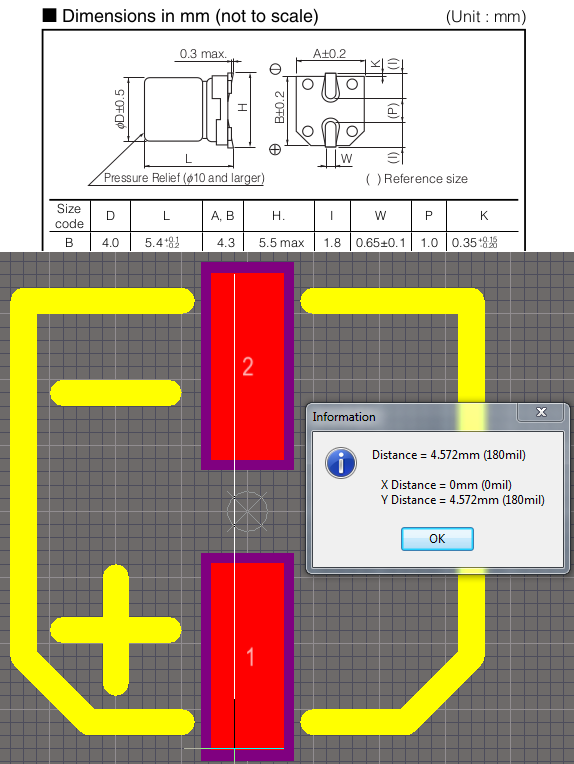
\includegraphics[width=10cm,keepaspectratio]{pcb/pol_cap_size_footprint_vs_specs.png}
\caption{Polarized capasitor footprint dimentions}
\label{figure:pol-cap-size-yo}
\end{center}
\end{figure}

The footprint for the polarized capacitor components were designed to match the component's outline, resulting in a footprint barely being large enough to contain the actual component~\vref{figure:pol-cap-size-yo}.

\begin{figure}
\begin{center}
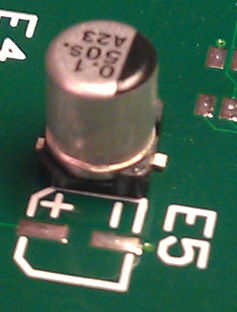
\includegraphics[width=5cm,keepaspectratio]{pcb/pol_cap_size_on_board.png}
\caption{Pads on footprint are smaller than pins of component}
\label{figure:pol-cap-size-board}
\end{center}
\end{figure}

This made soldering nontrivial.
See \vref{figure:pol-cap-size-board}.

To avoid this complication the pads on footprint should be designed to be larger than the pins so that the pads protrude beyond the actual component when it is placed on the PCB, resulting in simpler soldering.
